\section{Tecnologias}

\subsection{Apple Homekit}

O Apple Homekit não é uma aplicação por si só, é uma espécie de base de dados semelhante ao Passkit e ao Healthkit também desenvolvidos pela Apple. Todas estes ''kits'' são utilizados pelas respetivas aplicações, neste caso o Homekit tem a aplicação Home, o PassKit tem o Passbook e o HealthKit o Health. 

O Homekit neste caso tem como função armazenar uma coleção de dispositivos relativos a casas inteligentes, oferecendo ainda funcionalidades mais avançadas como \textit{triggers}, onde é possível configurar um grupo de ações a executar com base em certos \textit{triggers}, como a hora, a localização do utilizador ou com base nos dados de algum dispositivo. Por exemplo, é possível configurar o sistema de modo a que ele ligue as luzes e abra a porta principal quando o utilizador estiver nas imediações da casa, ou até, ligar ou desligar o aquecimento a uma certa hora do dia. 

O Homekit possui também integração com a Siri, o assistente pessoal presente nos sistemas operativos da Apple, o que permite controlar os dispositivos registados no Homekit através de comandos de voz, como por exemplo, ''Siri fecha a porta da garagem''.

\subsubsection{Arquitetura}

Os dados no Homekit são estruturados da seguinte forma hierárquica:
\begin{itemize}
    \item Homes - são a unidade base de dados, que representam uma casa do utilizador. Um utilizador pode possuir várias casas geograficamente afastadas ou até dividir a sua casa em duas, como por exemplo, casa principal e anexo.
    
    \item Rooms - representam as salas ou quartos de uma casa. As salas no Homekit apenas possuem um nome que as identifica, como ''sala'' ou ''cozinha'', de maneira a que se possam executar comandos deste tipo: ''ligar as luzes da sala''.
    
    \item Acessories - são os dispositivos ou acessórios instalados nas casas e registados em salas específicas. Caso os acessórios não sejam registados em nenhuma sala, o Homekit coloca-os num ''default room'', um local especial para dispositivos sem uma sala específica.  
    
    \item Services - são os serviços oferecidos por um dispositivo, como por exemplo, um serviço para ligar a luz de uma lâmpada. Os dispositivos podem também ter serviços internos, como um atualizador de sistema.
    
    De notar que um único dispositivo pode oferecer vários serviços controlados pelo utilizador. Uma porta pode ter um serviço para a fechar e outro serviço para a abrir.
    
    \item Zones - são agrupamentos opcionais de salas, como por exemplo, ''1º andar'' ou ''garagem''. As zonas, tal como as salas, possuem apenas um nome. As zonas permitem ao utilizador utilizar comandos como, ''Siri, liga as luzes do 1º andar'', que irá ligar todas as luzes das salas do 1º andar.
\end{itemize}

\begin{figure}[H]
  \centering
        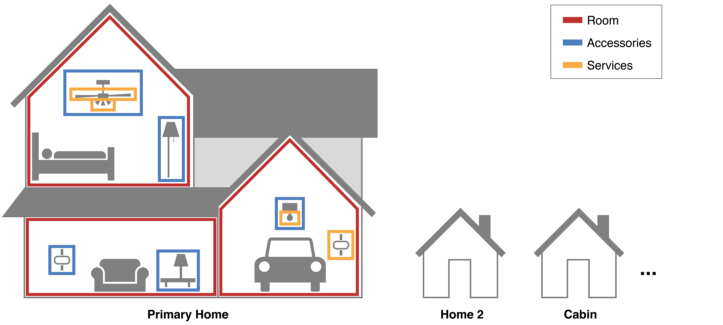
\includegraphics[scale=0.56]{img/homekit-layout.png}
  \caption{Arquitetura base dos elementos do Homekit}
\end{figure}

De seguida, um exemplo dos interfaces que demonstram os controlos do Apple Home, a aplicação que complementa o Homekit.

\begin{figure}[H]
  \centering
        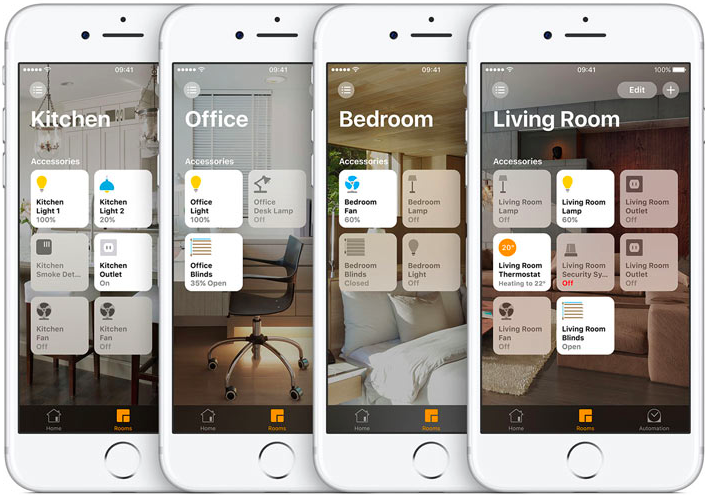
\includegraphics[scale=0.65]{img/homekit.png}
  \caption{Exemplo de interfaces gráficas do Apple Home}
\end{figure}

\subsubsection{API e interoperabilidade}

A API oferecida pelo Homekit permite o controlo total da base de dados do utilizador mediante a autorização do mesmo. Além disto, apenas aplicações revistas pela Apple e distribuídas na AppStore é que podem aceder à API do Homekit. Isto não é entrave nenhum ao desenvolvimento no entanto, uma vez que o XCode, o ambiente de desenvolvimento da Apple, possui um módulo de simulação, onde é possível adicionar dispositivos de testes, para testar a funcionalidade de aplicações ''Homekit enabled''. Resumidamente, tudo o que é possível fazer através da aplicação Home, é possível através desta API programaticamente.

De notar, que a API possui apenas um SDK para Swift ou Objective-C, portanto, o desenvolvimento nesta tecnologia só pode ser feito no ecossistema da Apple, o que é um ponto a menos na interoperabilidade desta tecnologia.

\subsection{Android Things}

O Android Things, originalmente chamado de Google Brillo, é um projeto orientado à ''Internet of Things'' desenvolvido pela Google, que tem como objetivo fornecer um sistema operativo para sistemas embebidos assim como um protocolo de comunicação, chamado Weave, para comunicarem com a cloud e dispositivos móveis.

Este projeto é uma versão básica do sistema operativo Android, possuindo apenas os serviços ''core'' do mesmo, de maneira a que possua uma utilização de memória bastante reduzida, sendo ideal para sistemas embebidos, e tendo todas as ferramentas do SDK Android e interfaces programáticos de acesso aos serviços da Google.

Todos os dispositivos utilizando o Android Things podem e devem ser conectados aos serviços cloud da Google, para que estejam sempre com as últimas atualizações dos serviços do sistema operativo. Além disso, os sistemas da Google recolhem constantemente informações do funcionamento dos dispositivos, via o protocolo Weave, e assim é possível aos programadores monitorizarem várias métricas de todos os seus dispositivos, como por exemplo, crash reports.

\begin{figure}[H]
  \centering
        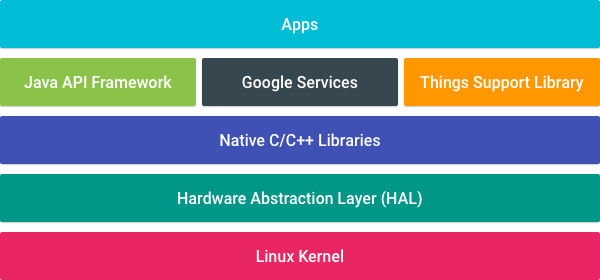
\includegraphics[scale=0.5]{img/platform-architecture-and-things.png}
  \caption{Arquitetura base do Android Things}
\end{figure}

\subsubsection{Weave}

O Weave é um protocolo de comunicação orientado à IoT, que permite que dispositivos desta área possam comunicar com smartphones e a cloud. O protocolo tem como objetivo abstrair as funções dos dispositivos IoT de modo a que possam ser reutilizado por várias aplicações e serviços web.

Este protocolo utiliza JSON como formato e a transmissão pode ser feita em HTTPS ou em XMPP. Além disso, este protocolo é protegido com SSL/TLS e a autenticação de dispositivos é feita utilizando OAuth 2.0 nos servidores de autenticação da Google. Utilizando este esquema de autenticação, a Google pode possibilitar a partilha destes dispositivos entre diferentes utilizadores, um pouco semelhante à partilha de documentos do Google Drive.

O Weave tem como objetivo fornecer um meio de comunicação entre dispositivos, smartphones e a cloud. A integração na cloud é um ponto muito forte, uma vez que com esta tecnologia aplicações poderão interagir com os dispositivos dos utilizadores, depois da autorização dos mesmos. 

\begin{figure}[H]
  \centering
        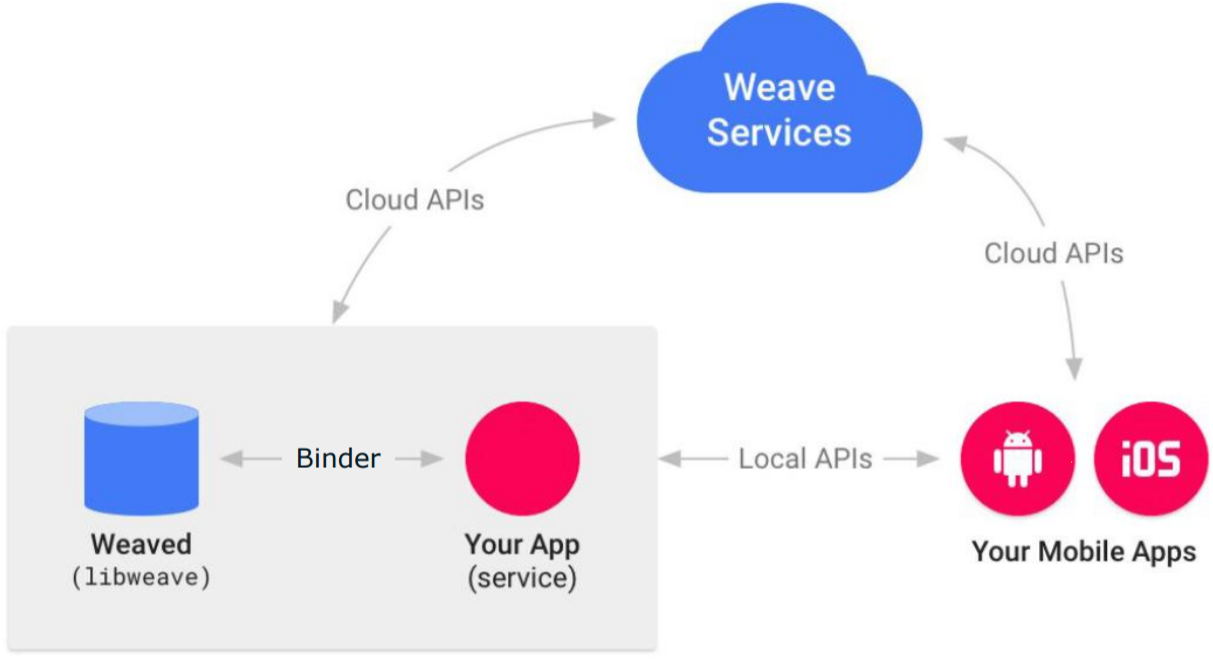
\includegraphics[width=\textwidth]{img/weave1.png}
  \caption{Arquitetura detalhada do Weave}
\end{figure}

De seguida, uma descrição das funcionalidades do Weave que se destacam:

\begin{itemize}

\item \textbf{Auto-configuração} - instalação de novos dispositivos podem ser feitas através de dispositivos Android (telemóveis) onde o utilizador efetua a autenticação do dispositivo e é redirecionado para a página da aplicação, caso o dispositivo a tenha.
    
\item \textbf{Monitorização de dispositivos} - através do portal do programador dos serviços Google, é possível analisar estatísticas dos dispositivos que utilizam Weave, nomeadamente, número de dispositivos online, distribuição de versões, distribuição de modelos de dispositivo, comandos enviados por hora.
    
\item \textbf{Over-the-air updates} - esta funcionalidade apenas funciona em dispositivos que utilizem o sistema operativo Brillo e consiste na atualização automática de dispositivos a partir do portal do programador da Google.
   
\item \textbf{Crash reports} - os programadores podem consultar o número de crashes ocorridos nos seus dispositivos assim como o número de utilizadores afetados e um log detalhado do crash em si.
    
\item \textbf{Dev Console} - é possível interagir com dispositivos protótipos, podendo testar comandos Weave sem ter que construir uma aplicação cliente. Muito útil para testar a fazer debug dos dispositivos antes de os colocar em produção.

\item \textbf{Home Assistant} - utilizando os serviços cloud do Weave, é possível fazer integração com o Home Assistant da Google, uma inteligência artificial que pode ser comandada com comandos voz. Desta maneira, o utilizador pode controlar os seus dispositivos através da sua própria voz, sem ter que recorrer à utilização física das aplicações.
\end{itemize}


\subsubsection{API e Interoperabilidade}

O Weave possui uma API que pode ser utilizada quer por dispositivos, quer por aplicações clientes nos dispositivos móveis ou até browsers web no desktop. Os utilizadores devem autorizar o acesso das aplicações clientes aos seus dispositivos, e depois disso, as aplicações clientes podem então interagir com os serviços do utilizador. O \textit{libweave} possui wrappers em várias linguagens nomeadamente Java e Go, além da versão original em C/C++.

Quanto ao Android Things, este oferece os serviços core do sistema operativo Android via o SDK em Java do mesmo, tal como se fosse uma aplicação mobile, mas apenas com os serviços core, não possuindo serviços como os contactos, telefone, mensagens, entre outros. O SDK providencia em vez disso, interfaces para acesso a serviços da Google, nomeadamente:

\begin{itemize}
\item \textbf{Chromecast} - serviço de streaming de telemóveis, tablets e computadores para dispositivos com suporte a esta tecnologia, por exemplo, sistemas de som ou televisões;
\item \textbf{Google Drive} - serviço de armazenamento de arquivos e edição de documentos;
\item \textbf{Firebase} - plataforma cloud da Google para suporte ao desenvolvimento de aplicações, contendo várias funcionalidades como: \textit{analytics}, \textit{crash reporting}, base de dados tempo real, configuração remota de aplicações e armazenamento de ficheiros;
\item \textbf{GoogleFit} - plataforma de monitorização de saúde e \textit{fitness} que recolhe dados de várias aplicações e dispositivos do utilizador para elaborar um perfil do utilizador com a sua performance em várias atividades físicas;
\item \textbf{Instance ID} - serviço de validação de aplicações para Android, iOS ou extensões do navegador Chrome. Esta API permite gerar tokens para autenticar o acesso a recursos \textit{server side}. Este mecanismo garante que os recursos \textit{server side} possam ser apenas acedidos pelas aplicações clientes registadas neste serviço;
\item \textbf{Awareness and Location} - esta API utiliza os sensores presentes no dispositivo para obter informações sobre os utilizadores das mesmas assim como o ambiente em geral;
\item \textbf{Nearby} - este serviço expõe métodos de \textit{publish} e \textit{subscribe} baseados na proximidade. Dispositivos próximos podem então recorrer a esta API para efetuarem comunicação em tempo real. Este serviço permite também efetuar \textit{service discovery}, sendo possível reconhecer dispositivos na rede local.
\item \textbf{Places} - através deste serviço é possível aceder a varias informações sobre locais no mundo, distribuídos por categorias, podendo por exemplo, localizar supermercados num raio de 5km à volta do utilizador;
\item \textbf{Mobile Vision} - esta API é um serviço de reconhecimento facial, podendo identificar rostos humanos em fotos, vídeos e transmissões em direto. A API também é capaz de identificar elementos detalhados dos rostos humanos, detetando se uma pessoa esta de olhos fechados ou a sorrir por exemplo.
\end{itemize}

O sistema operativo pode ser instalado numa gama de placas de prototipagem selecionadas, como o Intel Edison ou o Raspberry Pi 3, mas também pode ser compilado e instalado em qualquer tipo de dispositivo.

O projeto situa-se em \textit{open-beta}, e pode ser acedido via o portal para programadores da Google \cite{android-things}.

\subsection{Eclipse SmartHome}

O EclipseSmart Home é uma framework para o desenvolvimento de produtos direcionados a casas inteligentes. É “open-source” e completamente livre ao público geral. A filosofia dos criadores desta framework assenta no facto que a única maneira de ter uma framework verdadeiramente extensível, aberta e preparada para a evolução constante deste mercado, é tornando a mesma “open-source”, para que qualquer indivíduo possa contribuir e para que não existam exclusividades proprietárias, como acontece noutras frameworks da área. 

Esta framework é compatível com qualquer tipo de sistema que consiga correr a JavaVirtualMachine. É uma framework OSGi 4.2+, sendo compatível com por exemplo o RaspberryPI, e um número de outras placas de prototipagem. Isto é uma grande vantagem no desenvolvimento, já que é possível efetuar o desenvolvimento para esta framework em MacOS, Linux e Windows.


O SmartHome é orientado aos fabricantes de hardware, que podem preparar os seus dispositivos para serem compatíveis com soluções SmartHome, aos fabricantes de aplicações, que podem desenvolver as suas soluções para serem baseadas no SmartHome e tendo assim compatibilidade com uma vasta gama de dispositivos já existentes no mercado. Por fim, os programadores, que podem desenvolver extensões para o SmartHome que serão compatíveis com qualquer tipo de produto que utilize o SmartHome como base e até poderão disponibilizar estas extensões em plataformas comerciais.

De acordo com o inquérito \cite{ieeesurvey} a programadores realizado pela IEEE sobre tecnologias utilizadas nesta área, o Eclipse SmartHome é a tecnologia mais utilizada, provando a grande comunidade por detrás desta framework.

Esta framework é bastante completa, sendo compatível com grande parte das soluções IoT existentes no mercado, e é além disso, completamente extensível. Existem vários \textit{plugins} desenvolvidos pela comunidade que oferecem compatibildade para todo o tipo de dispositivos.

De seguida, um pequeno resumo sobre as \textit{features} desta framework:

\begin{itemize}
\item \textbf{Configuração Textual} - é possível configurar os dispositivos presentes num sistema a base de ficheiros texto. O Eclipse SmartHome possui uma DSL própria, e oferece ao mesmo tempo uma aplicação para editar ficheiros que utilizam esta linguagem, o SmartHome Designer, que oferece mecanismos \textit{auto-completion} e de validação.

\item \textbf{Áudio e Voz} - o SmartHome oferece mecanismos de \textbf{\textit{Text-to-speech}} e de \textbf{\textit{Speech-to-text}} que permitem aos utilizadores, teoricamente, controlar o sistema utilizando comandos voz, utilizando o \textbf{\textit{Human Language Interpreter}} desenvolvido pela Eclipse. De momento, os idiomas suportados são o Inglês e o Alemão.

\item \textbf{Rest API} - a framework oferece uma Rest API que permite a serviços externos interagirem com o sistema via pedidos HTTP. A API permite listar e configurar dispositivos e ainda oferece suporte a \textit{Server Sent Events}\cite{sse}, para que as aplicações clientes possam ser notificadas em tempo real de alterações dentro do sistema.

\item \textbf{Regras} - essencial para qualquer sistema de \textit{home-automation}, com esta framework é possível definir regras que automatizam o sistema, por exemplo, fechar os estores quando o vento está acima de uma certa velocidade ou fechar as portas da garagem a partir de uma certa hora.

\newpage

A framework deixa definir estas regras textualmente, um exemplo:

\begin{Verbatim}
ON item_id state changed 
    IF item_id.state == desired_value 
        THEN item_id2.state = desired_value2 
\end{Verbatim}

\item \textbf{Internacionalização} - todos os elementos desta framework podem ser internacionalizados, desde que sejam providenciados os coretos ficheiros, neste caso, ficheiros de propriedades i18n Java.

\item \textbf{Interfaces Gráficos} - esta framework oferece bastantes elementos para o desenvolvimento de interfaces gráficos, como icones, widgets, entre outros. Além disso, existem mecanismos para definir interfaces através de ficheiros texto. Estes ficheiros são \textit{sitemaps}, que define que dispositivos e que informações sobre os mesmos e mecanismos de controlo aparecem no interface gráfico.

\begin{figure}[H]
  \centering
        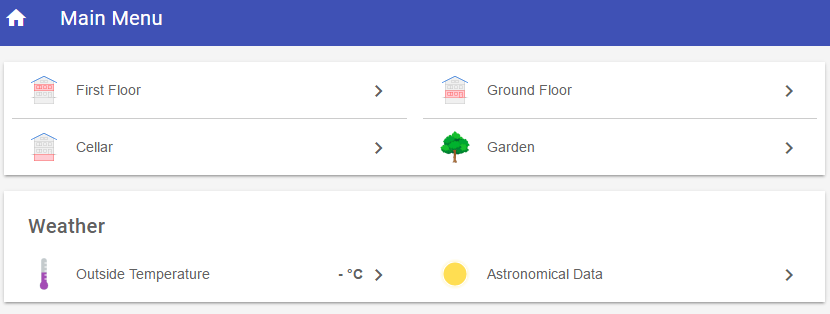
\includegraphics[scale=0.7]{img/smarthome-gui.png}
  \caption{Exemplo da interface gráfica do SmartHome}
\end{figure}

\begin{figure}[H]
  \centering
        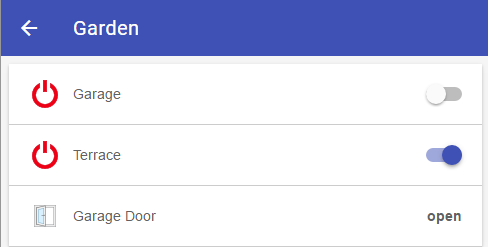
\includegraphics[scale=0.7]{img/smarthome-garden.png}
  \caption{Exemplo dos controlos da divisão ''garden''}
\end{figure}

\end{itemize}

\subsection{Arquitetura}

O Eclipse SmartHome diferencia a sua arquitetura em dois paradigmas, o paradigma físico, que representa o estado físico do sistema, ou seja, dos dispositivos e serviços ligados aos SmartHome, e o paradigma funcional, que representa as funcionalidades do sistema disponíveis ao utilizador. Resumidamente, o paradigma físico é útil para a configuração do sistema e resolução de problemas, e o paradigma funcional é útil para a interação entre os utilizadores e o sistema.

A nível aplicacional, o paradigma físico é representado por \textbf{Things} e o paradigma funcional é representado por \textbf{Items}. 

\textbf{Things} são entidades que podem ser adicionadas fisicamente ao um sistema e que podem fornecer várias funcionalidades ao mesmo tempo. \textbf{Things} podem ser tanto equipamentos reais que se podem adicionar um sistema como serviços web, como um serviço de meteorologia por exemplo. As \textbf{Things} oferecem a sua funcionalidade através de \textbf{Channels}.

\textbf{Items} representam as funcionalidades utilizadas pelas aplicações, neste caso, os interfaces gráficos e a lógica de automação. Estes \textbf{Items} são porventura ligados a \textbf{Thing Channels}  através de links. 

De seguida, os tipos de \textbf{Items} presentes nesta framework:

\begin{table}[H]
\centering
\resizebox{\textwidth}{!}{\begin{tabular}{lll}
\hline
\multicolumn{1}{|l|}{\textbf{Itemname}}         & \multicolumn{1}{l|}{\textbf{Description}}                           & \multicolumn{1}{l|}{\textbf{Command types}}           \\ \hline
\multicolumn{1}{|l|}{Color}         & \multicolumn{1}{l|}{Color information (RGB)}                           & \multicolumn{1}{l|}{OnOff,IncreaseDecrease,Percent,HSB}           \\ \hline
\multicolumn{1}{|l|}{Contact}       & \multicolumn{1}{l|}{Item storing status of e.g. door/window contacts}  & \multicolumn{1}{l|}{OpenClose}                                    \\ \hline
\multicolumn{1}{|l|}{DateTime}      & \multicolumn{1}{l|}{Stores date and time}                              & \multicolumn{1}{l|}{}                                             \\ \hline
\multicolumn{1}{|l|}{Dimmer}        & \multicolumn{1}{l|}{Item carrying a percentage value for dimmers}      & \multicolumn{1}{l|}{OnOff, IncreaseDecrease, Percent}             \\ \hline
\multicolumn{1}{|l|}{Group}         & \multicolumn{1}{l|}{Item to nest other items / collect them in groups} & \multicolumn{1}{l|}{}                                             \\ \hline
\multicolumn{1}{|l|}{Number}        & \multicolumn{1}{l|}{Stores values in number format}                    & \multicolumn{1}{l|}{Decimal}                                      \\ \hline
\multicolumn{1}{|l|}{Player}        & \multicolumn{1}{l|}{Allows to control players (e.g. audio players)}    & \multicolumn{1}{l|}{PlayerPause, NextPrevious, RewindFastforward} \\ \hline
\multicolumn{1}{|l|}{Rollershutter} & \multicolumn{1}{l|}{Typically used for blinds}                         & \multicolumn{1}{l|}{UpDown, StopMove, Percent}                    \\ \hline
\multicolumn{1}{|l|}{String}        & \multicolumn{1}{l|}{Stores texts}                                      & \multicolumn{1}{l|}{String}                                       \\ \hline
\multicolumn{1}{|l|}{Switch}        & \multicolumn{1}{l|}{Typically used for lights (on/off)}                & \multicolumn{1}{l|}{OnOff}                                        \\ \hline
                                    &                                                                        &                                                                  
\end{tabular}}
\caption{Tipos de items do SmartHome}
\label{smarthometypes}
\end{table}

Os vários dispositivos e serviços web são então disponibilizados na framework recorrendo a \textbf{Bindings}, que disponibilizam estes serviços através dum conjunto de \textbf{Things}.

Além disso, o SmartHome alia este mecanismo com o seu serviço de \textbf{Inbox \& Discovery}, que permite à framework procurar dispositivos compatíveis na rede e a adicionar-los a uma \textbf{Inbox}, para posterior configuração.

No entanto, a verdadeira configuração dos sistemas são feitos através de configuração textual, onde se podem especificar as \textbf{Things} dum sistema, juntamente com as suas configurações, como por exemplo, endereços IPs e afins. Além disto, também são especificados que tipos de \textbf{Items} irão ser retirados dos \textbf{Thing Channels}

De seguida, um pequeno exemplo de como a \textbf{Binding} do YahooWeather funciona.

A \textbf{binding} disponibiliza o serviço de meterologia sobre o formato de um \textbf{thing}, que tem como parametros de configuração a \textbf{location}, local a analisar, e o outro parâmetro é o \textbf{refresh}, que define a taxa de atualização em segundos dos dados da meteorologia. 

Esta \textbf{thing} possui então 3 \textbf{channels}:

\begin{tabular}{lll}
\textbf{Channel ID}                        & \textbf{Item Type}                   & \textbf{Description}                                                     \\ \hline
\multicolumn{1}{|l|}{temperature} & \multicolumn{1}{l|}{Number} & \multicolumn{1}{l|}{The current temperature in degrees Celsius} \\ \hline
\multicolumn{1}{|l|}{humidity}    & \multicolumn{1}{l|}{Number} & \multicolumn{1}{l|}{The current humidity in \%}                 \\ \hline
\multicolumn{1}{|l|}{pressure}    & \multicolumn{1}{l|}{Number} & \multicolumn{1}{l|}{The current pressure in millibar (hPa)}     \\ \hline
\end{tabular}

Comparando esta situação a um paradigma orientado a objeto, os \textbf{channels} são semelhantes a métodos e a \textbf{thing} representa um objeto, com os \textbf{items} a atuar quase como tipos de dados.\\\\

De seguida, a configuração textual deste exemplo:

\paragraph*{Things}
\noindent
Configuração do serviço de meteorologia. 

\begin{Verbatim}
yahooweather:weather:berlin [ location=638242 ]
\end{Verbatim}

\paragraph*{Items}
\noindent
Definição do \textbf{Item} \textit{Temperature}, que irá conter a temperatura retornada pelo serviço de meteorologia.

\begin{Verbatim}
Number Temperature 
    "Outside Temperature" 
        { channel="yahooweather:weather:berlin:temperature" }
\end{Verbatim}

\paragraph*{Sitemap}
\noindent
Definição do interface gráfico associado a este exemplo. Neste caso iremos ter um menu chamado \textit{Main Menu} e um elemento com o valor presente no \textbf{Item} \textit{Temperature}

\begin{Verbatim}
sitemap demo label="Main Menu"
{
	Frame {
		Text item=Temperature
	}
}
\end{Verbatim}


